 
\chapter{Introduction to Semantic Assistants}

\section{Overview}
The \sa project aims to bring natural language processing (NLP)
techniques directly to end users by integrating them with common
desktop applications, such as word processors, email clients, or Web
browsers. To facilitate this integration, a service-oriented
architecture (Figure~\ref{fig:arch}) has been developed that allows to
integrate (desktop) clients with NLP services implemented in the GATE
framework.\footnote{GATE, \url{http://gate.ac.uk}} 

For the general motivation, design, and background on the \sa project,
please read the information on the \sa Web site\footnote{Semantic
  Assistants,
  \url{http://www.semanticsoftware.info/semantic-assistants}} and the
contained references first \citep{giwi08,aswc08}. This document only
describes the installation and use of the developed system.

\begin{figure}[t]
  \centering
  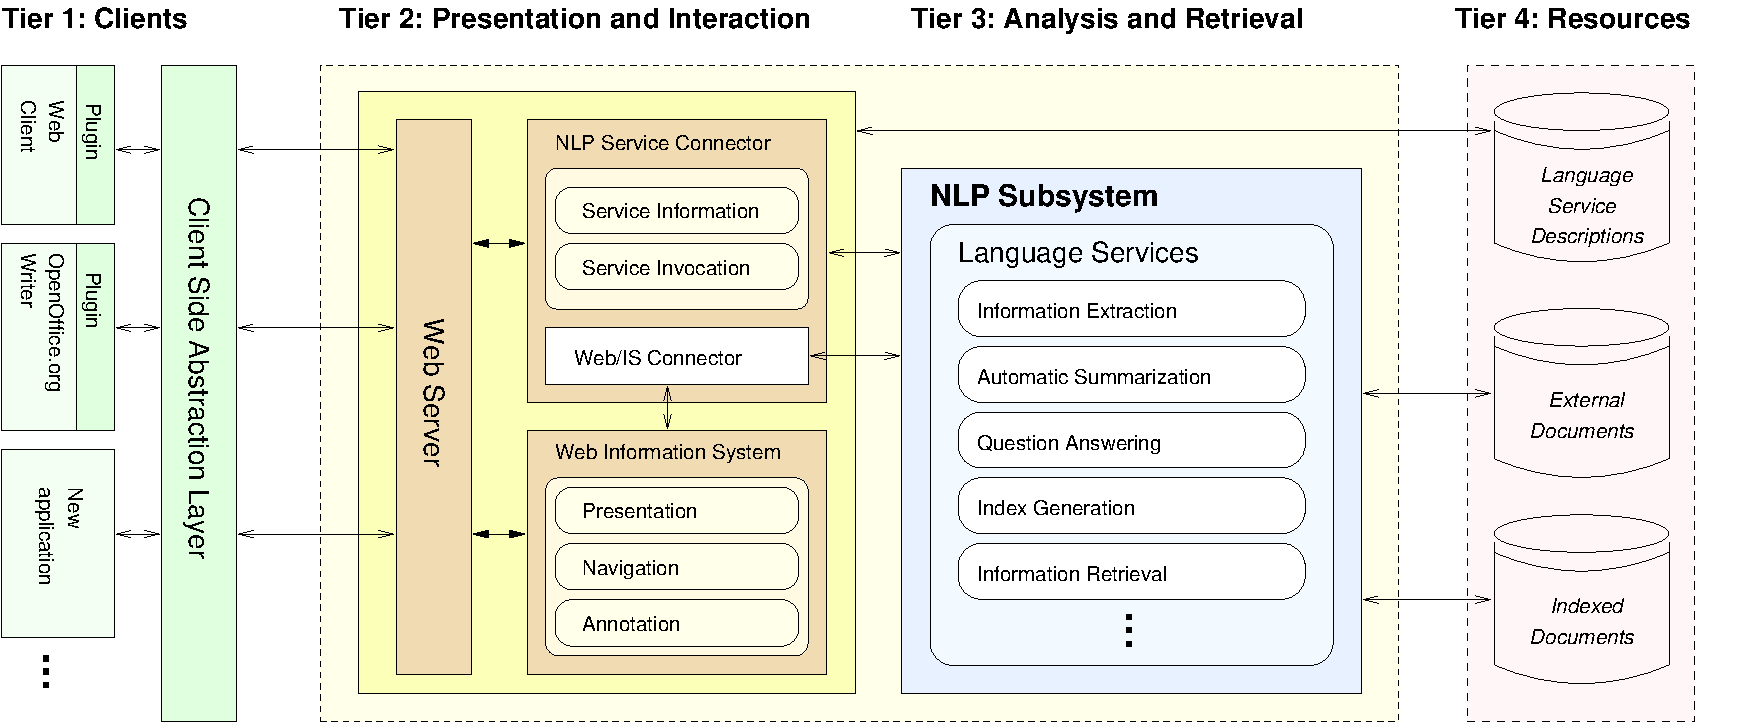
\includegraphics[width=\textwidth]{pictures/arch}
  \caption{The \sa architecture}
  \label{fig:arch}
\end{figure}

\section{How to read this documentation}
To deploy \sa, we recommend you first read this overview chapter.
Then, consult the following parts of this documentation:

\begin{description}
\item[End Users:] Please refer to the server installation guide
  (Chapter~\ref{chap:inst}) and the client guides in
  Chapter~\ref{chap:clients}.

\item[Language Engineers:] If you want find out how to integrate a new
  NLP service, please refer to Section~\ref{sec:nlpservices} and
  Section~\ref{sec:owl} for documentation on the OWL service
  descriptions.

\item[Plug-in Developers:] Please first read the background material
  (Web site, papers). Then refer to the developers' notes in
  Chapter~\ref{chap:dev}.
\end{description}

\section{Architectural Overview}
\label{sec:implementation}
This section gives an overview over the current version of the Semantic
Assistants architecture, as shown in Figure~\ref{fig:arch}:

\paragraph{Tier 1} of the architecture consists of client applications
and a \emph{Client-Side Abstraction Layer (CSAL)}. Currently, there
are two example clients distributed with the system, a simple
command-line client for testing purposes and a plug-in for the
OpenOffice.org \emph{Writer} word processor. The client-side abstraction
layer consists partly of hand-written Java classes that provide
common client-side functionality, partly of automatically generated
Java classes. The communication between client and server is
implemented by means of W3C Web services.\footnote{Web Services Architecture, see
  \url{http://www.w3.org/TR/ws-arch/}} 

\paragraph{Tier 2} of the architecture consists of a \emph{Web server}
and the \emph{NLP Service Connector}. The Web server used by default
in the architecture is the Java~6 embedded Web server.  The NLP
Service Connector currently integrates the GATE framework for NLP. It
is responsible for a number of tasks, including communication with the
client, reading and querying the language service descriptions,
running requested language services, and generating response messages.

\paragraph{Tier 3} is the NLP subsystem. At present, only the GATE
framework is supported (future work might integrate additional
frameworks, such as UIMA).  It makes use of the GATE API in order to
assemble language services, store them in a permanent way, and invoke
them when they are requested by a client.

\paragraph{Tier 4} is the resource tier.  Here we have the language
service descriptions, which are authored in the Web Ontology Language
(OWL).  Tier~4 further contains external documents, which the NLP
subsystem must be able to access. Finally, we possibly have
pre-indexed documents as part of the resources tier. For indexing,
GATE uses Apache's Lucene indexer\footnote{Apache Lucene, see
  \url{http://lucene.apache.org/}} as a subsystem, and allows us,
through its API, to create and access indices.


\section{System Components}
\label{sec:syscomp}
The implementation of the Semantic Assistants architecture currently comes
with the following components:

\begin{description}
\item[Server:] The server is the core of the architecture.  It
  communicates with the clients through the CSAL on one hand and
  the NLP framework through the NLP Service Connector on the other.
  At present, the architecture only contains a connector for
  GATE. However, it was explicitly designed to allow an easy
  integration of other frameworks (for example, UIMA). For describing
  available services, we use ontology-based (OWL) service
  descriptions. As a service-oriented architecture (SOA), every
  service is automatically available to all clients connected to the
  architecture, using standard WSDL\footnote{Web Services Description
    Language (WSDL), see \url{http://www.w3.org/TR/wsdl}}) interface
  descriptions.

\item[Client-Side Abstraction Layer (CSAL):] Our top goal was to make
  it as easy as possible for client (plug-in) developers to integrate
  NLP functionality. As clients should be able to connect to the
  architecture entirely by ``local'' means, we provide an
  \emph{abstraction layer}, named CSAL, which is located on the client
  side and performs the actual communication with the server.

  Apart from the communication functionality, the CSAL also provides
  common client-side functionality, i.e., useful data types and
  methods that are frequently required when integrating NLP into
  desktop clients.

\item[Clients:] Two example clients come with the architecture: a
  command-line client and a plug-in for the OpenOffice.org Writer word
  processor. 

\item[Example Resources:] NLP functionality is provided to clients
  through Web services. To match clients with suitable services
  (depending on language, formats, etc.), each NLP service comes with
  a semantic service description in OWL format. Three example service
  descriptions are included in the current distribution: an
  information extraction (IE) service that detects persons and locations
  (using GATE's ANNIE pipeline), an IR service (using the Yahoo PR)
  and a compound service, which combines the IR and the IE
  service. These should help you in defining your own NLP services
  that you deliver to your end users (e.g., summarization,
  question-answering, domain-specific NLP services).

\item[Documentation and Online Resources:] Apart from this guide, a
  number of publications on the \sa are available
  online,\footnote{\sa,
    \url{http://www.semanticsoftware.info/semantic-assistants}} as
  well as a discussion forum for support.
\end{description}


% \begin{figure}
%   \centering
%   %\vspace*{-9mm}
%   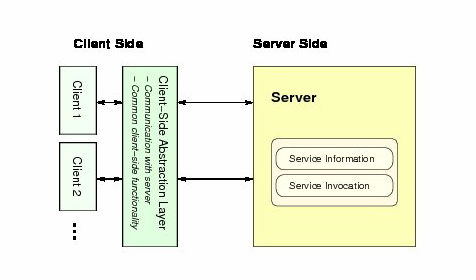
\includegraphics[width=0.6\textwidth]{pictures/abstraction.jpg}
%   \caption{We introduce a client-side abstraction layer}
%   \label{fig:abstraction}
%   %\vspace*{-0.4cm}
% \end{figure}



